% !TEX root = ./proposal.tex
\documentclass[12pt,a4paper]{article}

% --- Packages ---
\usepackage[utf8]{inputenc}
\usepackage[margin=1in]{geometry}
\usepackage{titlesec}
\usepackage{setspace}
\usepackage{graphicx}
\usepackage{subcaption}
\usepackage{booktabs}
\usepackage[backend=biber, style=numeric, sorting=none]{biblatex}
\usepackage{hyperref}
\usepackage{xcolor}

% --- Bibliography Link ---
\addbibresource{references.bib}

\title{\textbf{Master's Thesis Research Proposal: NMF + ML framework to detect DPV signatures in noisy marine environments where standard methods fail}}
\author{Your Name}
\date{January 2026}

\begin{document}

\maketitle
\onehalfspacing

\section*{ABSTRACT}
NMF + ML framework to detect DVP signatures in noisy marine environments where standard methods fail.

\section{INTRODUCTION}
Underwater passive acoustics monitoring (PAM) is a key enabling technique for marine security with
applications such as vessel or diver detection and identification of submerged vehicles.... The emergence
of quiet, motorized assistance for divers has introduced new challenges for security monitoring.

Diver propulsion vehicles (DPVs) are compact - electric motorized systems that assist scuba divers to
cover long distances underwater. Unlike vessels that radiate broadband cavitation noise, DPVs produce
weak, narrowband tonal signatures from brushless DC motors that are easily masked by the ambient
underwater noise. The similarities between the DVP's acoustic signatures to small, motorized vessels
make it challenging to detect DPVs, and to the best of our knowledge no work has offered robust approach
to identify between vessel and DPV noise.... To address this gap, we develop detection strategy that relies
on the stability of the DVP's tonal lines.

In this work, we identify DPV noise from vessel noise by taking a physics-information machine learning
(PIML) approach. PIML integrates domain knowledge and physical constraints into machine learning
models, allowing the algorithm to leverage both data-driven learning and expert understanding of the
system. In context of the underwater detection, PIML enables the incorporation of knowledge of DPV
acoustic characteristics specifically the narrowband tonal properties of electric motors while letting the
machine learning component learn from real-world data variations.... Our goal is for a robust approach that
is insensitive to the DVP make and the marine environment.

We will implement our solution over embedded hardware deployed on a buoy. Continuously recording
and real-time detection using a single hydrophone will demonstrate the effectiveness of our solution in
real sea conditions. Tests will take place in both deep and shallow waters.... We will measure the
performance of our solution in terms of the detection and false alarm rate as well as based on the
response time.

\section{OBJECTIVES}
Our work explores the question "Can we acoustically identify the underwater radiated noise (URN) of DPVs
from that of vessels?”. To answer this question, we will develop a method to detect DPVs by PAM while
avoiding the false detection of vessel's URN as DPV-related noise. We will design an algorithm that
classifies DVP and vessel noises. We aim for a probability of detection exceeding 90\% and a false alarm
rate under 5\% for a signal-to-noise ratio (SNR) power values below 0 dB.... These goals exceed the
performance of current vessel detection schemes as reviewed next.

\section{LITERATURE REVIEW}
Current PAM-related detection methods typically fall into two categories: classical energy detectors (e.g.,
DEMON, Band-pass) or machine learning. Energy detectors rely on the identification of the vessel's
cavitation modulation or the identification of periodicities in the signal. Conversely, machine learningapproaches rely on the identification of characteristic features in the signal.... A variety of methods explored ways to identify the URN of vessels.

\begin{itemize}
    \item Common methods for vessel detection apply cyclostationary form detectors.... The URN of electric
vehicles such as DVP have similarities and dissimilarities to the URN of motorized non-electric vessels.
    \item On top of the cavitation and thruster-based URN components, the URN of electric motors includes
harmonics determined by the shape of the electric motor.... The challenge in properly modeling the URN
of electric vessels leads to the choice of ML-based approaches for detection of marine vessels noise
and signal Spectrogram.
    \item Current Machine learning solutions are mostly geared for the detection of the vessel's broadband
noise.... To the best of our knowledge, no current solution is offered for classifying DPV from vessels.
The limitation in detecting electric vessels calls for a better understanding of the nature of the electric
vessel's noise.
\end{itemize}

\section{METHODOLOGY}
Our solution for the URN detection of DVPs focuses on the combination of ML in the detection process of
identifying tonal lines in the soundscape. This \colorbox{yellow}{[TBD: elaborate]} PIML approach lets the ML find the stable
factor of the DVP's tonal line, while the expectation about narrowband harmonics in the DVP's URN is
utilized to verify detection. We will measure our performance by taking an emulation approach.

Based on our preliminary data collection work that accumulated both DVP's URN and regular vessel noise
from the same recorder type, we will explore sensitivities to DVP type and noise level by synthetically
combining recorded signals with recorded ambient noise… An implementation of our approach will be
tested in several sea trials by implementing our code over an existing buoy system deployed by our lab in
Eilat, the Red Sea, and using real DVPs in controlled experiments. A picture of this buoy system with its two self-made hydrophones is shown in Fig.~****1. \colorbox{yellow}{[TBD: add here picture of the buoy from Eilat]}

\section{NOVELTY AND SIGNIFICANCE}
To the best of our knowledge, this will be the first solution to distinguish between the URN of DPVs and
standard surface vessels. While recent research has explored the application of NMF for acoustic source
separation and signal enhancement \cite{chanNonNegativeMatrixFactorizationConvolutional2019} as well as the URN of electric vessels \cite{kitaAdvancesPassiveAcoustic2022},
our approach is unique by combining ML to identify the stability factor within the NMF framework. This way,
we avoid the need to model the narrowband characteristics of the detected DVPs.... The choice of our
approach was developed through our preliminary work to collect URN of DVPs of different types as
discussed next.

\section{PRELIMINARY WORK}
DVP sea experiments were conducted in two distinct marine environments: Haifa, Israel using the Seacraft
GO!, and Zapadni Greben, near Silba Island Croatia using the Suex VRX DVPs. Both trails were conducted
during June and July of 2025. The DVP's URN was recorded using an icListen HF ALTA acoustic recorder
unit. The acoustic data was sampled at 128KHz and included continuous recordings of .wav files. The
experimental setup included both hydrophones attached to mooring and mobile scenarios with recordersattached to a scuba diver (shown in Figure 7). A total of 500 minutes of DVP URN were recorded at
distances, varying between 1m up to 1,000m. A separate control dataset of 1,000 hours of verified DVPfree noise was collected using the same recorder set as was used for the DVP recording. The noise-only
dataset was collected some 4 km west of the Haifa port's shipping lanes. Raw data was segmented based
on timestamps to isolate the DPV transacts.... The dataset collected during these preliminary trials
provides a ground truth dataset for performance evaluation.

\subsection{Trial procedures and environments}
The Haifa experiments were conducted in 18-25 m water depth using a stationary hydrophone attached to a mooring line. The hydrophone was at ~10m depth, at the same depth of the drivers' dives. The scuba divers used the Seacraft GO! scooter on prescribed tracks with a typical sequence used a low-speed outbound leg (about 0.7 m/s) followed by a higher-speed return leg, so that the same path was sampled at different SNR conditions.

In Silba (July 2025), a Suex VRX DPV was recorded in a quieter Adriatic environment with similar water depths and buoy/weights/hydrophone setup but with reduced shipping noise. Several trials with different route geometries (linear, circular, serpentine), speeds (about 0.7-2.5 m/s), and maximum ranges up to 1000 m were performed. Some runs intentionally coincide with marine traffic (ferry and small boat as shown in Figure 6) to create realistic interference scenarios where DPV tonal signatures overlap in time and
frequency with larger vessels. A description of dive site and the GPS track of one of the routes taken, is shown in Figure \ref{fig:silba-1k}.

\begin{figure}[h]
        \centering
        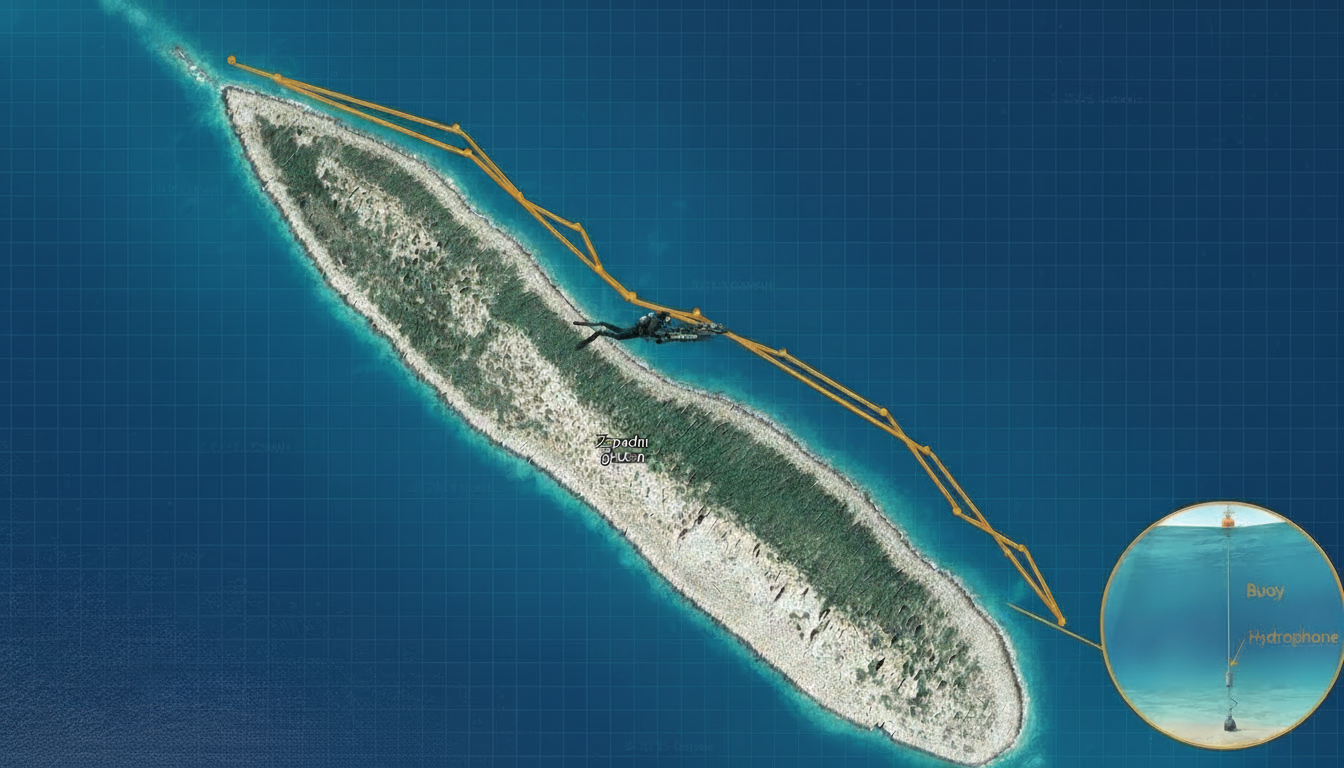
\includegraphics[width=\textwidth]{images/silba-1k.png}
        \caption{The GPS tracking of the 1k transacts near Zapadni Greben, Croatia and of the recorder and bouy setup.}
        \label{fig:silba-1k}
\end{figure}

Raw recordings were segmented using experiment logs and GPS tracks to isolate individual DPV and vessel passes. Time-frequency representations were computed with standard STFT parameters and used as input to Non-negative Matrix Factorization (shown in Figures \ref{fig:signal-spectrogram} \& \ref{fig:signal-spectrogram-with-nmf}). NMF decomposed the spectrograms
into a small number of spectral bases and their temporal activations, separating stable tonal components associated with DPVs from broadband ambience and transient interference (shown in Figures \ref{fig:nmf-basis} \& \ref{fig:nmf-coefficients}).
\colorbox{yellow}{[TBD: include some conclusions from what you already have]}

\begin{figure}[!h]
    \centering
    % Row 1
    \begin{subfigure}[b]{0.49\textwidth}
        \centering
        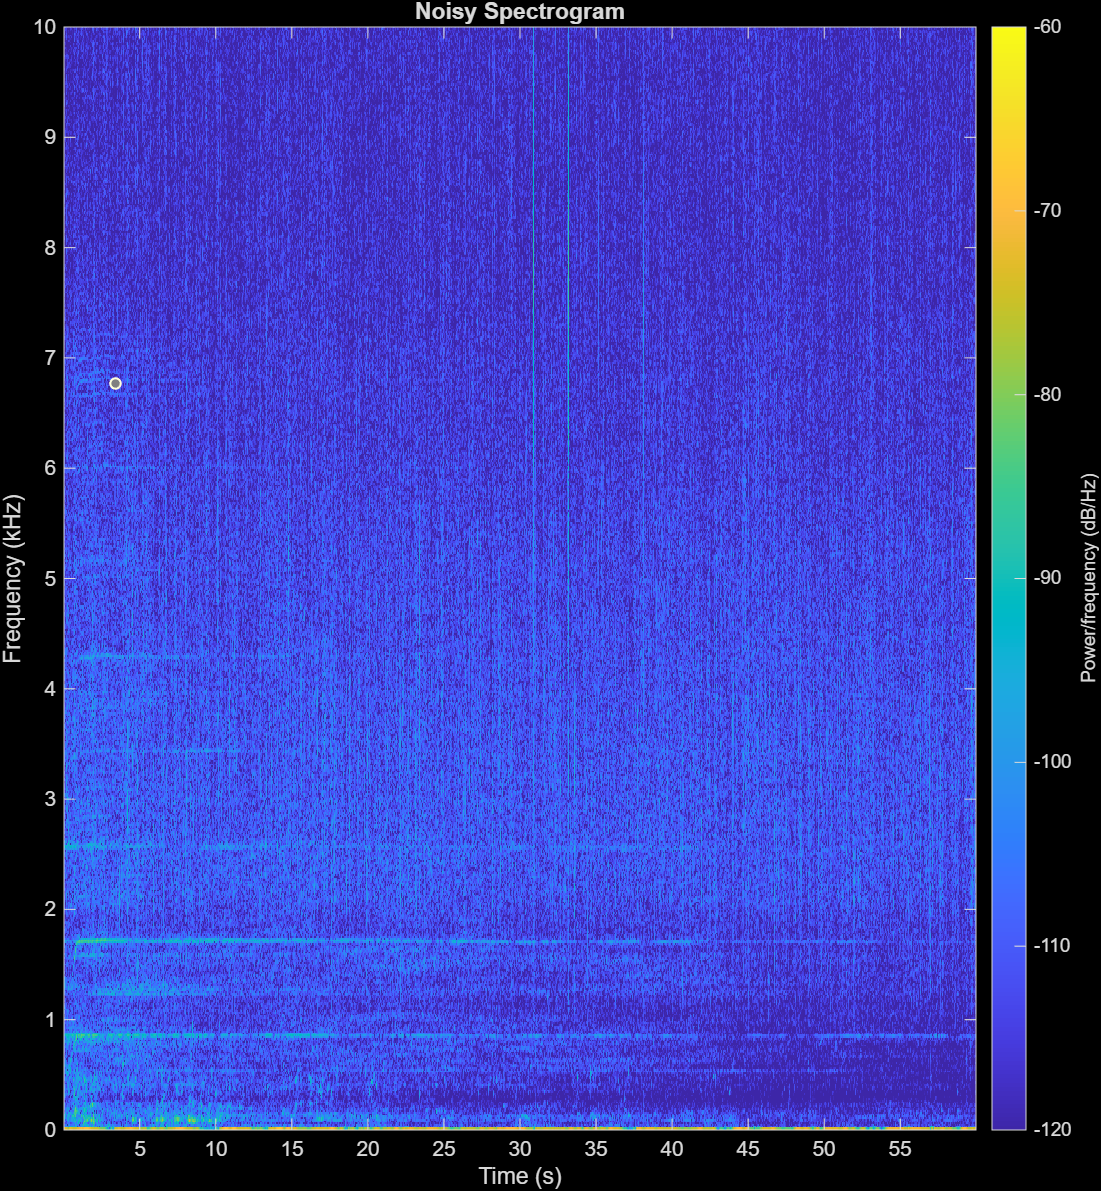
\includegraphics[width=\textwidth]{images/Noisy Spectrogram.png}
        \caption{Raw signal Spectrogram}
        \label{fig:signal-spectrogram}
    \end{subfigure}
    \hfill
    \begin{subfigure}[b]{0.49\textwidth}
        \centering
        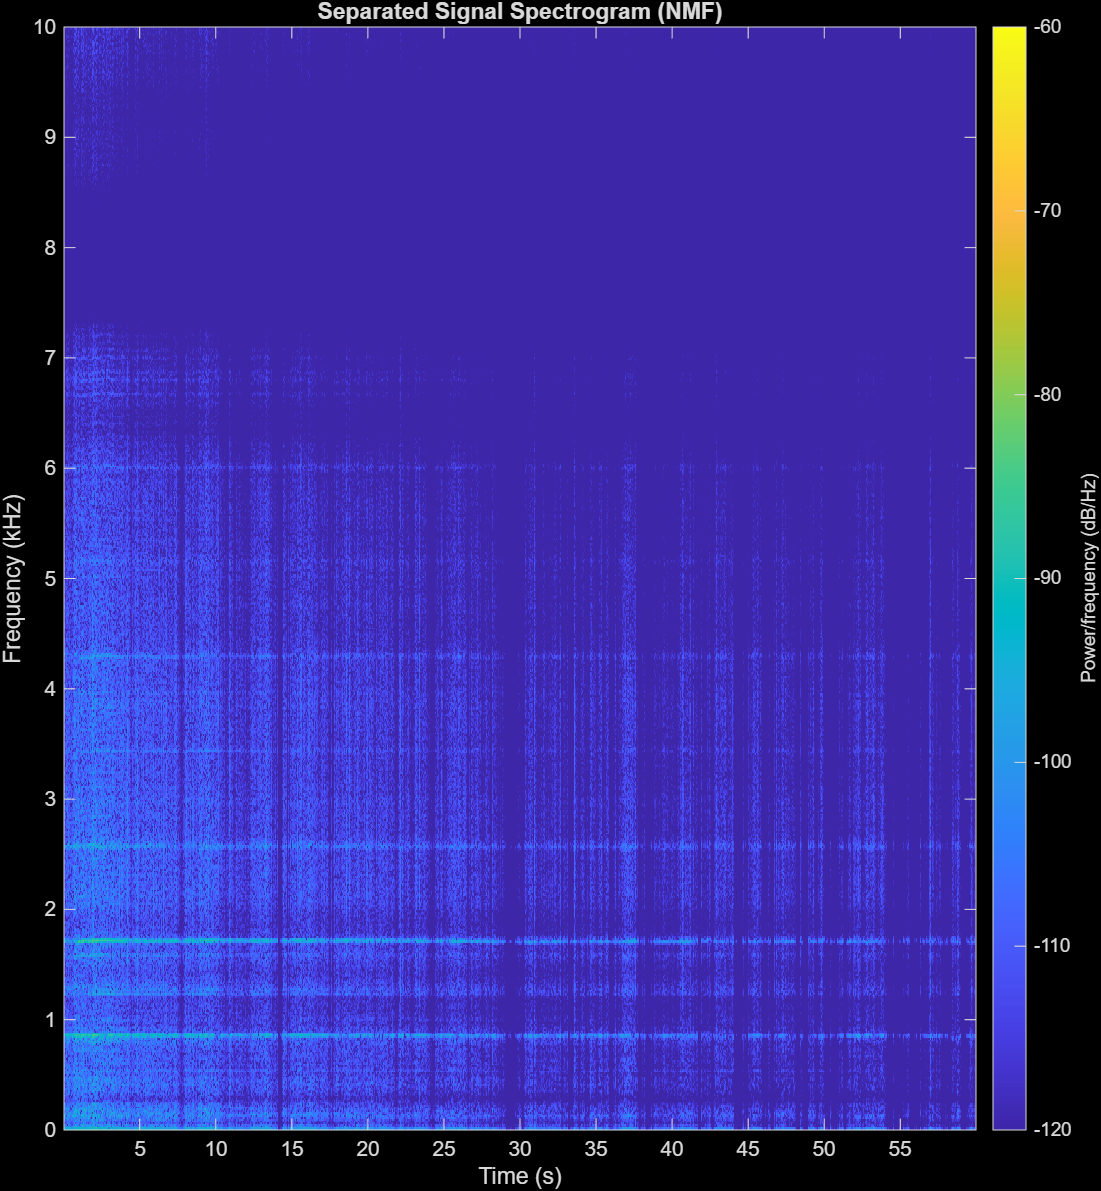
\includegraphics[width=\textwidth]{images/Separated Signal Spectrogram.png}
        \caption{Signal Spectrogram after applying NMF}
        \label{fig:signal-spectrogram-with-nmf}
    \end{subfigure}
    \caption{Overview of DPV acoustic signal Spectrogram and NMF separation results.}
    \label{fig:signal-spectrograms}
    \vspace{1em} % Spacing between rows
    
    % Row 2
    \begin{subfigure}[b]{0.98\textwidth}
        \centering
        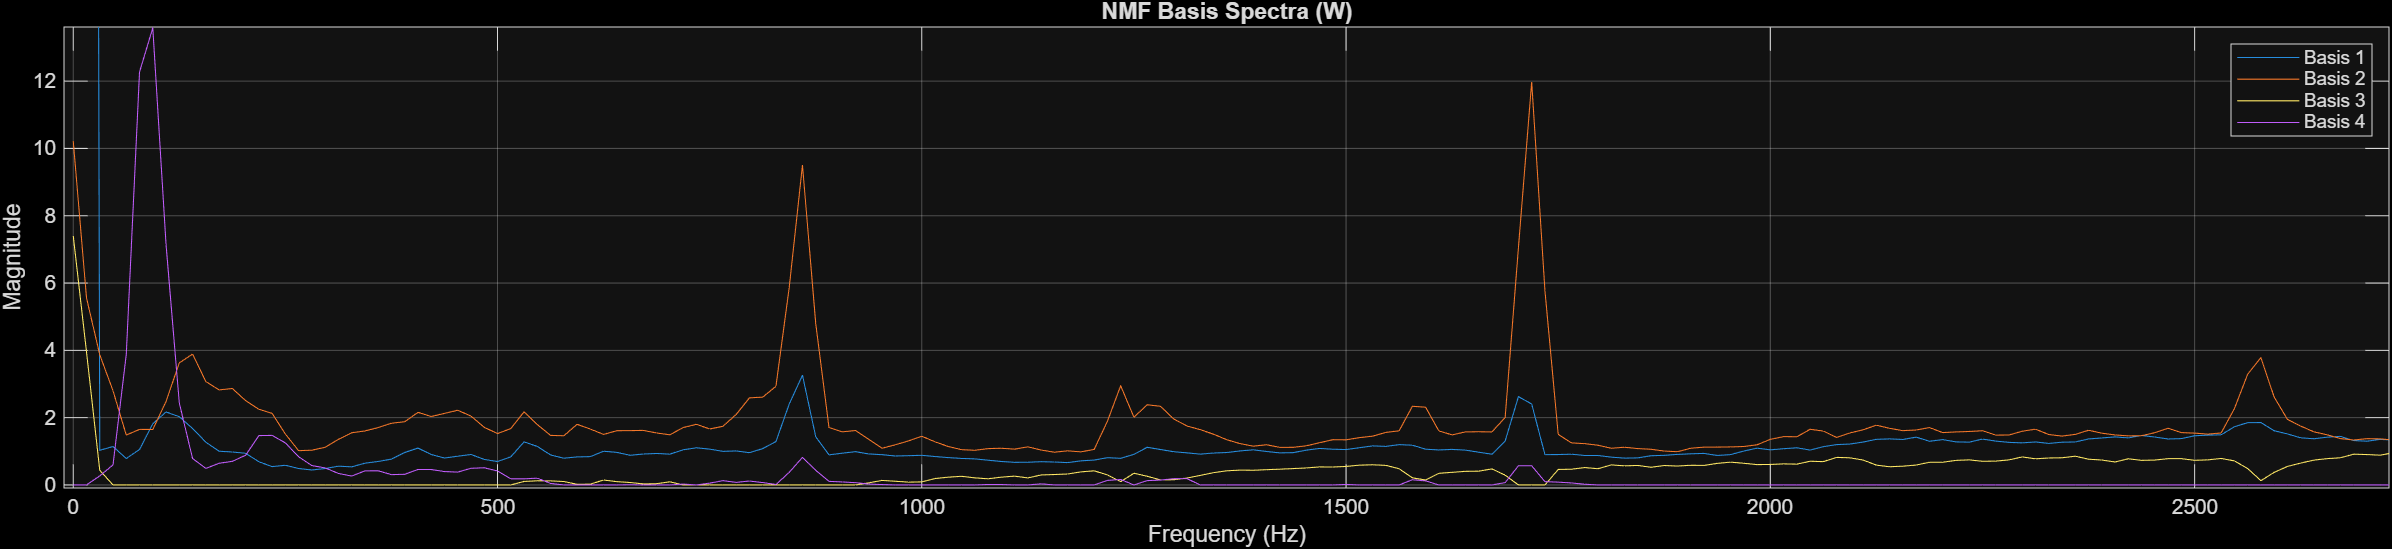
\includegraphics[width=\textwidth]{images/NMF-Basis.png}
        \caption{NMF tonal components (basis)}
        \label{fig:nmf-basis}
    \end{subfigure}
    \hfill
    \begin{subfigure}[b]{0.98\textwidth}
        \centering
        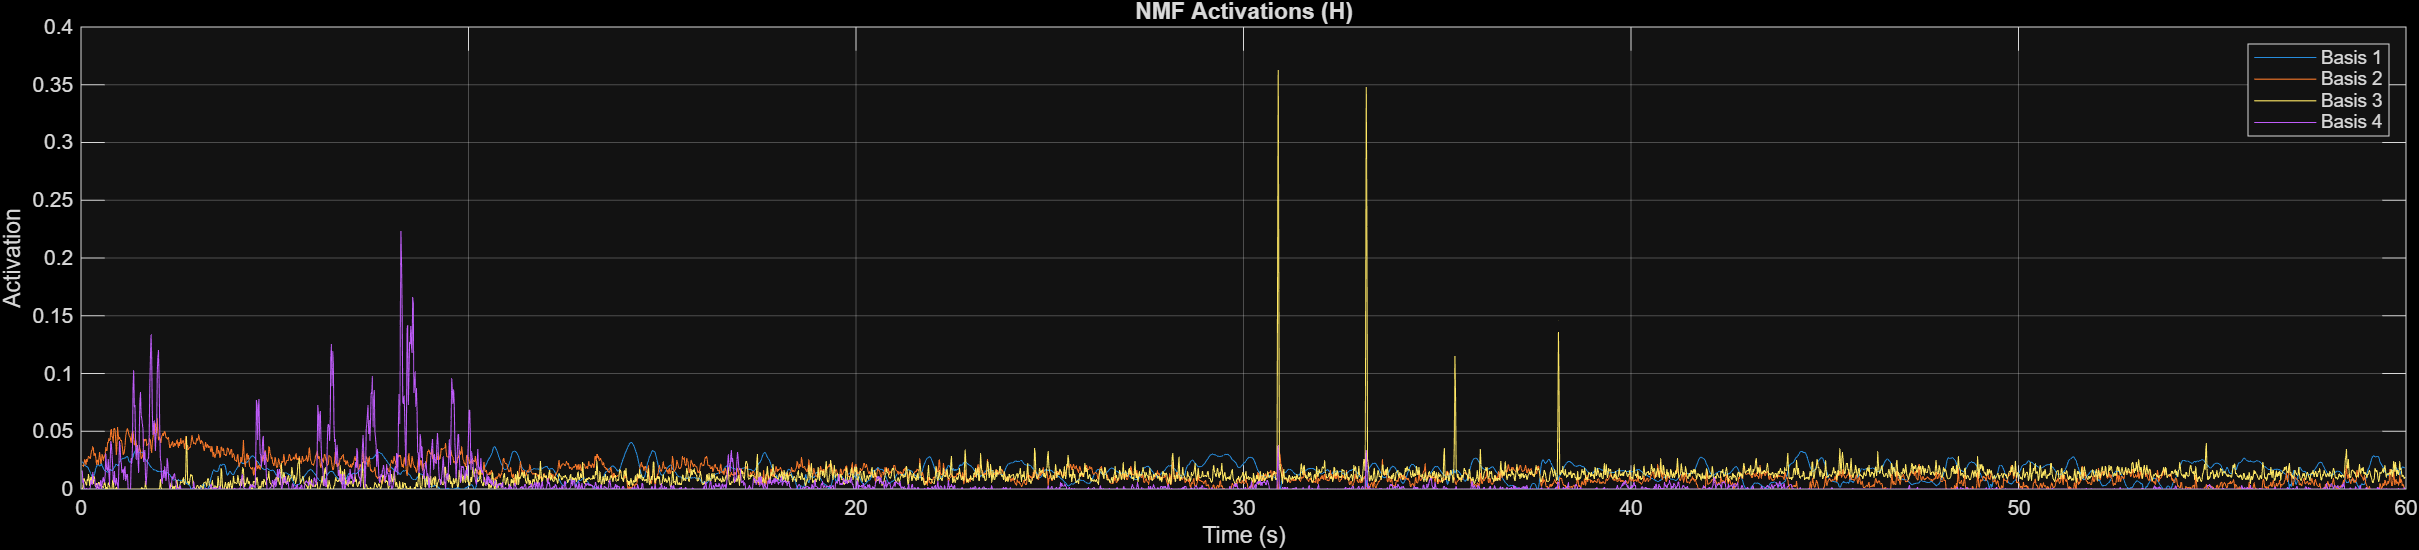
\includegraphics[width=\textwidth]{images/NMF-Activations.png}
        \caption{NMF Activation components (coefficients)}
        \label{fig:nmf-coefficients}
    \end{subfigure}    
    \caption{Overview of DPV acoustic signatures and NMF separation results (2x3 Grid).}
    \label{fig:nmf-components}
\end{figure}

\begin{figure}[htbp]
    \centering
    % Row 1
    \begin{subfigure}[b]{0.32\textwidth}
        \centering
        \includegraphics[width=\textwidth]{example-image-a}
        \caption{Description 1}
        \label{fig:img1}
    \end{subfigure}
    \hfill
    \begin{subfigure}[b]{0.32\textwidth}
        \centering
        \includegraphics[width=\textwidth]{example-image-b}
        \caption{Description 2}
        \label{fig:img2}
    \end{subfigure}
    \hfill
    \begin{subfigure}[b]{0.32\textwidth}
        \centering
        \includegraphics[width=\textwidth]{example-image-c}
        \caption{Description 3}
        \label{fig:img3}
    \end{subfigure}
    
    \vspace{1em} % Spacing between rows
    
    % Row 2
    \begin{subfigure}[b]{0.32\textwidth}
        \centering
        \includegraphics[width=\textwidth]{example-image-a}
        \caption{Description 4}
        \label{fig:img4}
    \end{subfigure}
    \hfill
    \begin{subfigure}[b]{0.32\textwidth}
        \centering
        \includegraphics[width=\textwidth]{example-image-b}
        \caption{Description 5}
        \label{fig:img5}
    \end{subfigure}
    \hfill
    \begin{subfigure}[b]{0.32\textwidth}
        \centering
        \includegraphics[width=\textwidth]{example-image-c}
        \caption{Description 6}
        \label{fig:img6}
    \end{subfigure}
    \caption{Overview of DPV acoustic signatures and NMF separation results (2x3 Grid).}
    \label{fig:2x3_grid}
\end{figure}

\subsection*{Summary of Experiments Conducted}
All recordings were done using the icListen HF ALTA hydrophone and recorder system, with a 128kb sampling frequency.
\begin{table}[h!]
\centering
\resizebox{\textwidth}{!}{
\begin{tabular}{lllllll}
\toprule
\textbf{Date} & \textbf{Location} & \textbf{Time (min)} & \textbf{Max Distance (m)} & \textbf{Speed (m/s)} & \textbf{Route Type} & \textbf{Type of Vehicle Used} \\ \midrule
12/06/2025 & Haifa, Israel & 31 & 500 & 0.7 & Circular & Seacraft Go! DVP\\
23/07/2025 & Silba, Croatia & 50 & 50 & 2.5 & Linear & Suex VRX DVP\\
24/07/2025 & Silba, Croatia & 34 & 600 & 0.7, 2.2 & Linear & Suex VRX DVP, including Ro-Ro Passenger Ferry noises \\
24/07/2025 & Silba, Croatia & 37 & 500 & 2.2 & Serpentine & Suex VRX DVP \\
25/07/2025 & Silba, Croatia & 25 & 1000 & 0.7, 2.2 & Linear & Suex VRX DVP \\
25/07/2025 & Silba, Croatia & 16 & 100 & 2.2 & Circular & Suex VRX + Boat \\ 
\colorbox{yellow}{TBD} & Haifa, Israel & \colorbox{yellow}{TBD} & & & & Haifa port multiple overlapping ship noises \\
\colorbox{yellow}{TBD} & Haifa, Israel & \colorbox{yellow}{TBD} & & & & Mid-sea, multiple ship noises \\
\bottomrule
\end{tabular}}
\end{table}



\section{TIMELINE}
\begin{table}[h!]
\centering
\begin{tabular}{lll}
\toprule
\textbf{Task} & \textbf{Deliveries} & \textbf{Due Date} \\ \midrule
Data collection & Varied datasets & Nov. 2025 \\
Literature survey & Comparison table & Dec. 2025 \\
Research proposal & Submission & Feb. 2026 \\
R \& D & NMF-ML pipeline results & June 2026 \\
Thesis submission & Final Thesis & Aug. 2026 \\
Thesis defense & Presentation & Oct. 2026 \\ \bottomrule
\end{tabular}
\end{table}

\printbibliography

\end{document}